\section{Unsere Lowlevel Extras}

Über unsere 3 Hauptfragen hinaus, entdeckten wir zusätzlich viele kleine "lowlevel" Cheats.
Diese wollen wir jetzt nacheinander kurz durchgehen und erklären.

\subsection{Cabbage Cheat}
Während dem Spielen merkt man schnell, dass man die Möglichkeit hat die Kohlköpfe, die in den Räumen verteilt sind,
in die Löcher zu schmeißen. 

\begin{figure}[H]
    \centering
    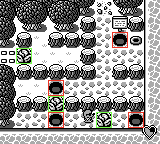
\includegraphics[width=0.5\linewidth]{Bilder/07-lowlevel_01.png}
    \caption{Raum 16}
    \label{fig:enter-label}
\end{figure}

Alle 5 Kohlköpfe erhält man neue Lebenspunkte dazu. \\

Wir fanden heraus das an der WRAM Adresse 0xce66 die Kohlköpfe gezählt werden die bereits in Löcher
geschmissen worden sind. An der Adresse 0x0000b48fc wird überprüft ob diese Zahl durch 5 teilbar ist.
Es sieht folgendermaßen aus:\\\\
if (mod\_5([0xce66] == 0)) \{ \\
\hspace*{2em} erhalte Heilung\\
\}\\

Und diese Modulorechnung kann man zum beliebigen Verändern, so dass das Spiel leichter oder schwerer wird.
In unserem Cheattool hat man die Option, es so einzustellen, das jeder Kohlkopf heilt.

\subsection{Invincibility}

WRAM Adresse 0xce52, speichert die Trefferpunkte des Maulwurfs. In der Funktion der Schadensberechnung,
an der Stelle 0x001d76df, wird dieser Wert um 1 verringert. Beim Überschreiben des Befehls z.B. mit 0x00, verliert man 
ab sofort keine Trefferpunkte mehr. 

\subsection{}

How was the question received, did interviewees struggle with a particular part
the most.
